\documentclass[10pt,twocolumn,letterpaper]{article}

\usepackage{cvpr}
\usepackage{times}
\usepackage{epsfig}
\usepackage{graphicx}
\usepackage{amsmath}
\usepackage{amssymb}
\usepackage{color}

% Plotting fun :D
\usepackage{tikz,pgfplots}

\newcommand{\preliminary}[1]{\textcolor{red}{#1}}

% Include other packages here, before hyperref.

% If you comment hyperref and then uncomment it, you should delete
% egpaper.aux before re-running latex.  (Or just hit 'q' on the first latex
% run, let it finish, and you should be clear).
\usepackage[pagebackref=true,breaklinks=true,letterpaper=true,colorlinks,bookmarks=false]{hyperref}

% \cvprfinalcopy % *** Uncomment this line for the final submission

\def\cvprPaperID{****} % *** Enter the CVPR Paper ID here
\def\httilde{\mbox{\tt\raisebox{-.5ex}{\symbol{126}}}}

% Pages are numbered in submission mode, and unnumbered in camera-ready
\ifcvprfinal\pagestyle{empty}\fi
\begin{document}

%%%%%%%%% TITLE
\title{What If Localization Worked?}

\author{First Author\\
Institution1\\
Institution1 address\\
{\tt\small firstauthor@i1.org}
% For a paper whose authors are all at the same institution,
% omit the following lines up until the closing ``}''.
% Additional authors and addresses can be added with ``\and'',
% just like the second author.
% To save space, use either the email address or home page, not both
\and
Second Author\\
Institution2\\
First line of institution2 address\\
{\tt\small secondauthor@i2.org}
}

\maketitle
%\thispagestyle{empty}

%%%%%%%%% ABSTRACT
\begin{abstract}
   Real world computer vision systems typically have some intrinsic value in their underlying business use. Serving the the right image in a search result ad might be worth \$0.001 and counting nuclear particles in material images might be worth \$10,000. In general, we want to build systems which produce sufficiently accurate results within a given budget. Although an interaction with human workers can improve accuracy in many algorithms, it also increases the cost. Most computer vision research focuses on purely automated algorithms, arguing that human labor is much too expensive to be included as subroutines in operational algorithms. In this work, we put this argument into perspective by investigating joint algorithms using computers and human labor. In particular, we focus on how different degrees of human involvement effect the algorithm's accuracies. We focus on the representative computer vision task of localization, however, our general methodology can similarly be applied to other tasks, e.g., Object Detection or Image Matching. We introduce several general strategies for combining existing computer vision algorithms with human labor, e.g. (To be filled). We evaluate our results on three reference data sets, i.e., UIUC Cars, Caltech Pedestrian and Street View House numbers, and show how the accuracy of the algorithms scale with varying degrees of human involvement. Finally, we provide an outlook on what computer vision applications become possible, if localization works.
\end{abstract}

%%%%%%%%% BODY TEXT
\section{Introduction}

\section{Localization}
\preliminary{
A place to describe
\begin{enumerate}
\item definition of what we understand it is
\item Where localization fits into a typical classification pipeline, which helps us motivate why we chose to focus on this problem in particular
\item state of the art
\item data sets
\item applications
\end{enumerate}
}

% Contributed by students:
\preliminary {
Object localization is one of the most obvious parts of any computer vision application. It involves two basic tasks namely semantic segmentation and object detection. Semantic segmentation is the task of labelling the pixels of an image depending on their semantic category while object detection produces a rough location (bounding boxes) of all the instances that belong to a set of objects of interest. Our research focuses more on object detection. Object detection allows us to count the number of objects precisely, which is not always possible from semantic segmentation.
Where does localization fit into a typical classification pipeline? This helps us motivate why we chose to focus on the problem of localization in particular( to be done)
These are some previously proposed papers on object localization using different techniques~\cite{localization01,localization02}. Although these papers provide various impressive techniques, we through our paper would like to improve upon the accuracy of the localization algorithm by incorporating HPU component with it.
}

\preliminary{
TODO: We're going to have to be extremely consistent with how we use our terminology. ``Detection''? ``Localization''? What's the difference? After we decide this (and this section is probably a good place to choose), we should do a Ctrl+F on all instances of both words and change them to match.
}


\section{Data Sets}
\preliminary{
\begin{enumerate}
\item in detail the picked data sets (refer to previous section why they are important.)
\item the measure of accuracy on those data sets
\end{enumerate}
}

\subsection{UIUC Cars}\label{sec:uiuc-cars}
For our first example, we chose the classic UIUC cars dataset, introduced in~\cite{agarwal2002learning,agarwal2004learning}. This dataset makes a particularly good baseline because it is well-established and because there is no recognition task after the initial detection/localization step. This dataset allows us to measure the performance of a simple single-class open-set detection task. The 550 positive samples in the test set are side views of cars, some of which are partially occluded, and the 500 negative training samples contain natural scenes, various other vehicles, etc.

On this dataset, performance is evaluated using standard precision/recall measures. F-measure and absolute number of false positives is also typically reported. In the single-scale case, the output bounding box is 100$\times$40px, and it counts as a correct detection if the center lies within a certain ellipse of the groundtruth's bounding box center. Since there may be many cars per image; statistics are aggregated over each individual car in the test set, not per image. The original parts-based representation in~\cite{agarwal2002learning} achieves about 77.58\% F-measure.

\preliminary{TODO: What is the state of the art?}


\subsection{Caltech Pedestrian Detection Benchmark}
The Caltech Pedestrian Detection Benchmark, introduced by~\cite{dollarCVPR09peds}, is a challenging pedestrian detection dataset. This set is several orders of magnitude larger than the UIUC~Cars set, containing 350,000 groundtruth pedestrian bounding boxes. The research that uses this dataset is summarized by~\cite{Dollar2012PAMI}.

To evaluate performance, this dataset asks authors to calculate a standard ROC curve of their detection results. However, in the open set ``self-driving car looking for pedestrians'' scenario, the amount of negative data is potentially infinite, which means plotting TP/TR is not very insightful. Instead, authors report miss rate versus number of false positives per image (``\emph{FPPI}''). This ROC curve is summarized as the ``\emph{log-average miss rate,}'' computed by averaging the miss rate at nine FPPI values along logarithmically-spaced intervals~\cite{Dollar2012PAMI}.

A detection counts as correct if its intersection-over-union score is greater than 0.5, meaning $\frac{\textsc{Area}(A \cap B)}{\textsc{Area}(A \cup B)} \geq 0.5$, where $A$ and $B$ are the detected and groundtruth bounding boxes respectively.

\subsection{Street View House numbers}
\cite{netzer2011reading}

\preliminary{Problem: The first paper that uses this dataset \cite{netzer2011reading} only reports classification accuracy, which is separate from the precision/recall tasks. It's unclear to me where they're assuming they have groundtruth segmentation and where they do not start from the crop set. We might be able to spin the story as ``Well what if it wasn't already solved? How would the existing algorithms perform if they didn't already have good crops? And how can we minimize this performance drop? This is a hard problem and nobody's thinking about it''. Or we could just pick a different dataset. Not sure.}

\preliminary{Question for you guys: did anyone find previous work that measures localization accuracy on this dataset?}

\section{Computer-Human Localization}
\preliminary{
A place to describe
\begin{enumerate}
\item Our different HCOMP algorithms
\item Examples
\item Evaluations (the famous plots we always talk about)
\end{enumerate}
}

\subsection{UIUC Cars}
% mjw note: here's just one example on how to include this kind of plot. Perhaps we should do this in excel instead? I'm open to anything, but keeping points+lines right in this document means we will never have to worry about keeping our plots in sync.
\begin{figure}[t]
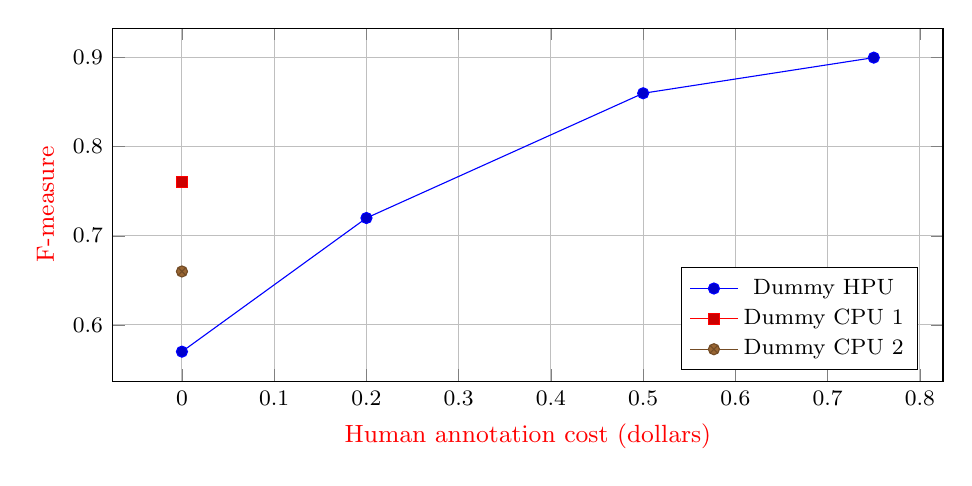
\begin{tikzpicture}
\begin{axis}[
    small, % changes font size, etc
    legend style={font=\footnotesize},
    width=\linewidth,
    height=0.5\linewidth,
    xlabel={\preliminary{Human annotation cost (dollars)}},
    ylabel={\preliminary{F-measure}},
    grid=major,
    legend pos={south east},
]

% Example of HPU line (DUMMY; REMOVE THIS
\addplot coordinates {
    (0, 0.57)
    (0.2, 0.72)
    (0.5, 0.86)
    (0.75, 0.9)
};
\addlegendentry{Dummy HPU}

% Example of a dummy CPU point
\addplot coordinates { (0, 0.76) };
\addlegendentry{Dummy CPU 1}
\addplot coordinates { (0, 0.66) };
\addlegendentry{Dummy CPU 2}
\end{axis}
\end{tikzpicture}
\caption{A graph showing how using crowdsourcing to adjust localization errors can improve accuracy. \preliminary{F-measure} is shown on the Y-axis and \preliminary{dollars} is shown on the X-axis. See Sec.~\ref{sec:uiuc-cars} for details.}
\end{figure}

\subsection{Caltech Pedestrians}
\subsection{Street view house numbers}


\section{Applications}
\preliminary{
A place to describe
\begin{enumerate}
\item Now that we've shown that we can improve accuracy, what other applications can we enable?
\item Graph that shows, human labour cost vs, profit of company/test... (the graph is generated by intersecting(or whatever maximization is needed between cost/accuracy and value/accuracy)
\end{enumerate}
}

\section{Conclusion}

%-------------------------------------------------------------------------


{\small
\bibliographystyle{ieee}
\bibliography{egbib}
}

\end{document}
